\documentclass[10pt,a4paper]{article}
\usepackage[utf8]{inputenc}
\usepackage[german]{babel}
\usepackage{mathrsfs}
\usepackage{amsmath}
\usepackage{amsfonts}
\usepackage{amssymb}
\usepackage{amsthm}
\usepackage[left=2cm,right=2cm,top=2cm,bottom=2cm]{geometry}
\usepackage{listings}
\usepackage{graphicx}

\begin{document}

\section{Aufgabe 7}

\subsection{Teil a}

\subsection{Teil b}

\subsection{Teil c}

\section{Aufgabe 8}

\begin{equation}
  T_{0}(x) = 1
\end{equation}
\begin{equation}
  T_{1}(x) = x
\end{equation}
\begin{equation}
  T_{2}(x) = 2x^{2} - 1
\end{equation}
\begin{equation}
  T_{3}(x) = 2x(2x^{2} - 1) - x
\end{equation}
\begin{equation}
  T_{4}(x) = 2x(2x(2x^{2} - 1) - x) - 2x^{2} + 1
\end{equation}
\begin{equation}
  T_{5}(x) = 2x(2x(2x(2x^{2} - 1) - x) - 2x^{2} + 1) - 2x(2x^{2} - 1) + x
\end{equation}
\begin{equation}
  T_{6}(x) = 2x(2x(2x(2x(2x^{2} - 1) - x) - 2x^{2} + 1) - 2x(2x^{2} - 1) + x) - 2x(2x(2x^{2} - 1) - x) + 2x^{2} + 1
\end{equation}
\begin{equation}
  T_{7}(x) = 2x(2x(2x(2x(2x(2x^{2} - 1) - x) - 2x^{2} + 1) - 2x(2x^{2} - 1) + x) - 2x(2x(2x^{2} - 1) - x) + 2x^{2} + 1) - 2x(2x(2x(2x^{2} - 1) - x) - 2x^{2} + 1) + 2x(2x^{2} - 1) - x
\end{equation}
\begin{equation}
  T_{8}(x) = 2x(2x(2x(2x(2x(2x(2x^{2} - 1) - x) - 2x^{2} + 1) - 2x(2x^{2} - 1) + x) - 2x(2x(2x^{2} - 1) - x) + 2x^{2} + 1) - 2x(2x(2x(2x^{2} - 1) - x) - 2x^{2} + 1) + 2x(2x^{2} - 1) - x) - 2x(2x(2x(2x(2x^{2} - 1) - x) - 2x^{2} + 1) - 2x(2x^{2} - 1) + x) + 2x(2x(2x^{2} - 1) - x) - 2x^{2} - 1
\end{equation}

\begin{lstlisting}
function y = tscheb (n, x)
  if n == 0
     y = ones(1, length(x));
  elseif n == 1
    y = x;
  else
    y = x .* 2 .* tscheb((n - 1), x) - tscheb((n - 2), x);
  endif
endfunction

hold on;

styles = ["y", "m", "c", "r", "g", "b", "y", "k", "m"];

x = -1:0.01:1;
for i = 0:8
  plot(x,
       tscheb(i, x),
       strcat(";T=", num2str(i), ";"),
       "Color", styles(i + 1),
       "LineWidth", 2);
endfor

hold off
\end{lstlisting}

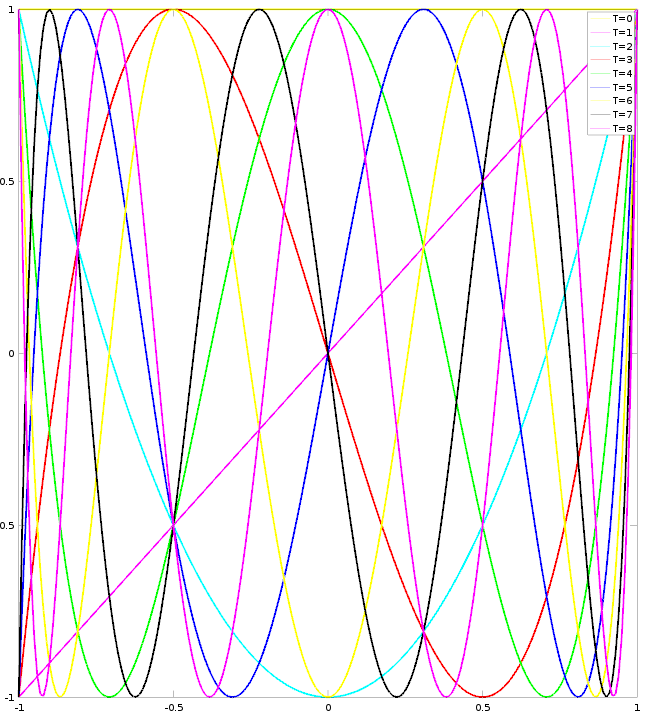
\includegraphics[width=250pt]{3_8.png}

\section{Aufgabe 9}

\subsection{Teil a}

\subsection{Teil b}

\subsection{Teil c}

\section{Aufgabe 10}

\end{document}